%!Mode:: "TeX:UTF-8"
\section{读书要点}
Q:阅读过哪些经典著作?

A:
\begin{description}
  \item[computer arch(2)] CSAPP, Computer Arch a quantitative approach
  \item[networking and os(2)]top-down approach,modern os
  \item[compilers(1)] dragon book
  \item[programming languages(3)] C++ Primer, Thinking in C++, thinking in Java
  \item[programming idoms and patterns(3)]Gof, programming pearls, Effective C++
  \item[alg(1)]Introduction to Algorithms
  \item[unix(2)]Unix Network Programming, APUE
  \item[Software engieering(2)]The Mythical Man-Month, Peopleware
  \item[non-classics]cryptography and security, big talk storage
\end{description}

\subsection{谭浩强}
谭浩强的风格缺陷:main函数签名不标准,改写静态字符串,域括号后面没有换行,声称要先在纸上写程序再输入。

\subsection{陈皓}
学习编程需要十年;程序员不是青春饭,30岁才入门。

\subsection{ACE}
一般地,I/O多路复用机制都依赖于一个事件多路分离器(Event Demultiplexer)。分离器对象可将来自事件源的I/O事件分离出来,并分发到对应的read/write事件处理器(Event Handler)。开发人员预先注册需要处理的事件及其事件处理器(或回调函数);事件分离器负责将请求事件传递给事件处理器。两个与事件分离器有关的模式是Reactor和Proactor。Reactor模式采用同步IO,而Proactor采用异步IO。可参考ACE源码。

ACE:connectors,pool。
ACE不仅仅是类库,而是通过模式协同在一起的一系列相关的类,如果对设计模式熟悉,那么会用助于学习ACE。





\section{代码阅读心得}

\begin{figure}
  \begin{center}
    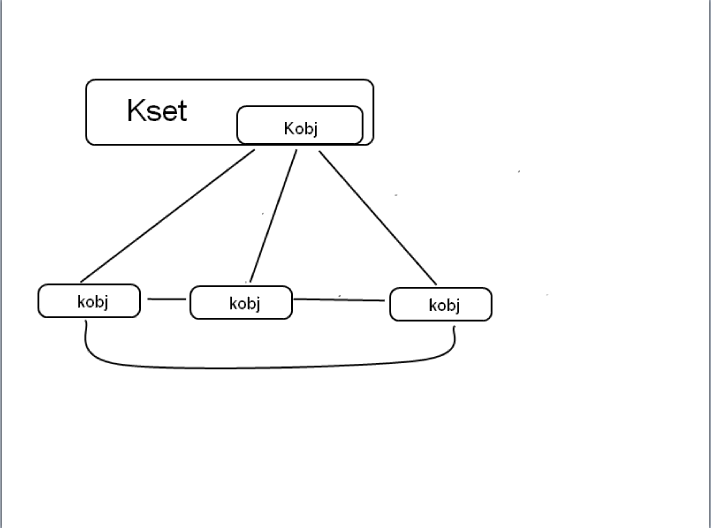
\includegraphics[keepaspectratio,width=0.36\paperwidth]{Pictures/kobject.png}
    \caption{kobject}
    \label{fig:kobject}
  \end{center}
\end{figure}

Nginx 1.0.14 约10万行代码(wc -l返回12万行)。Linux内核2.6.11版本约600万行。SGI STL约有2.4万行。


任何大型的代码都有预分配内存的思想。
Linux上有内存池,slab分配器。
Nginx有slab分配器和内存池。
SGI STL有两级内存分配器,参\ref{sec:memallocidioms}。

封装:struct中只有成员变量的封装,函数指针实际上也是作为变量进行封装。
成员函数封装,在C语言中相当于将操作同一结构的接口放在相同的接口文件中。

继承:ngx\_module\_t中的ctx字段,这种结构实现了继承,ngx\_module\_t相当于基类,而ctx指向派生类成员(包含在ngx\_http\_module\_t等结构中),虽然存储方式不同于C++的派生类。

多态:内核中多态的典型例子是虚拟文件系统。VFS可看做抽象基类,提供struct file\_operations相当于虚函数表。

重载(编译期多态):C语言中经常使用flag变量作为函数参数实现类似重载的效果。

组合:Linux内核中,kobject包含于kset,如图 \ref{fig:kobject}所示。
Linux和中定义有struct list\_head和struct rb\_node(类似于Nginx中的ngx\_queue\_t和ngx\_rbtree\_node\_t),用于生成双链表或红黑树,其他结构中包含它们可以看做组合。


复合型数据结构:如epoll中的epitem节点既属于红黑树,又属于双链表(因为包含list\_head)。前者用于被监控对象插入删除操作(epoll\_ctl),后者是为准备提交给用户的事件。
struct sched\_entity也同时包含struct rb\_node和list\_head。sched\_entity用于CFS(完全公平调度),task\_struct包含了一个sched\_entity。

特性萃取:trait模板、category类体系、重载函数体系。

Nginx用event对象的instance位来处理过期事件问题,instance是bool值,这样做有一定的概率还是会出错,应该改为一个较长的整形,每次
新分配连接时增一,这样,出错的概率极小。

Nginx的过滤模块链表并非链表,而是由各个模块的实现文件中的两个静态变量top和next实现的。




\section{开源代码阅读推荐}
\begin{description}
\item [LwIP] 轻量级协议栈,代码干净,注释详细
\item [memcached] 一套分布式的高速缓存系统, 用CRC-32计算键值后,将数据分散在不同的机器上,数据会以LRU机制替换掉
\item [Redis] Key-Value数据库,C编写,很短,可以全部看下。
\item [Lua] 一门动态语言,提供了一个虚拟机。几万行C代码,简洁优美
\item [uC/OS II]作为一个 RTOS 代码非常不多,分层也挺清楚的
\item [libevent] Libevent是一个轻量级的开源高性能网络库,使用者众多,c语言编写
\item [VxWorks] 美国WindRiver公司RTOS,VxWorks相对简单,模块清晰,代码风格良好
\item [Lucene] 搜索领域的经典项目,是一个高效的,是一个高效的 , 基于Java的全文检索库
\item [Sqlite] sqlite 是一款轻量级的、基于文件的嵌入式数据库,C编写
\item [Duplicity] Python项目。整合已有工具链,实现数据加密增量备份这一任务
\item [Quake III]雷神之锤,一个游戏
\item [trac] 基于Python的软件项目管理系统,拥有强大的bug管理 功能,并集成了Wiki 用于文档管理。它还支持代码管理工具Subversion ,这样可以在 bug管理和Wiki中方便地参考程序源代码
\item [其他] python,LVS,android SDK,BOOST,jdk,spring,openstack,MySQL
\end{description}

















